\documentclass[a4paper]{article}

\usepackage[UTF8]{ctex}
\usepackage[a4paper,margin=1in]{geometry}
\usepackage{graphicx}
\usepackage{float}
\usepackage{listings}
\usepackage{booktabs}
\usepackage{color}
\usepackage{indentfirst}
\setlength{\parindent}{2em}
\usepackage{zhnumber}
\usepackage{adjustbox}
\usepackage{subcaption}
\usepackage{amsmath}
\usepackage{amssymb}
\usepackage{enumitem}
\usepackage{lmodern}
\usepackage{inconsolata}
\usepackage{multirow}
\usepackage{tikz}
\usetikzlibrary{positioning}
\usepackage{fancyhdr}
\usepackage{hyperref}

% 配置lstlisting支持中文
\lstset{
    language=C,
    basicstyle=\footnotesize\ttfamily,
    breaklines=true,
    keywordstyle=\bfseries\color{blue},
    commentstyle=\itshape\color{green!50!black},
    stringstyle=\bfseries\color{red},
    numbers=left,
    numberstyle=\tiny\color{gray},
    frame=single,
    backgroundcolor=\color{gray!5},
    showstringspaces=false,
    keepspaces=true,
    tabsize=4,
    extendedchars=true,
    inputencoding=utf8,
    literate={，}{{\textcolor{green!50!black}{，}}}{1}
             {。}{{\textcolor{green!50!black}{。}}}{1}
             {：}{{\textcolor{green!50!black}{：}}}{1}
             {；}{{\textcolor{green!50!black}{；}}}{1}
             {（}{{\textcolor{green!50!black}{（}}}{1}
             {）}{{\textcolor{green!50!black}{）}}}{1}
             {【}{{\textcolor{green!50!black}{【}}}{1}
             {】}{{\textcolor{green!50!black}{】}}}{1}
}

\newcommand{\projname}{计算机图形学期末}
\newcommand{\reporttitle}{基于 OpenGL 的 3D 象棋系统个人报告}
\newcommand{\authorname}{马福泉}
\newcommand{\major}{计算机科学与技术}
\newcommand{\adviser}{陶钧}
\newcommand{\startdate}{2025年12月20日}
\newcommand{\labenddate}{2026年01月17日}

\pagestyle{fancy}
\fancyhf{}
\fancyhead[L]{\kaishu \projname}
\fancyhead[C]{\kaishu \reporttitle}
\fancyhead[R]{\kaishu \authorname}
\fancyfoot[C]{第 \thepage 页}
\renewcommand{\headrulewidth}{0.4pt}
\renewcommand{\footrulewidth}{0pt}


\begin{document}

% 封面
\begin{titlepage}
    \centering
    
\includegraphics[width=10cm]{img/SYSULogo.png}
    \vspace{1em}
    % 修改为换行并居中
    \par
    {\Large \kaishu
        \par
        \projname
        \par
    }
    \vspace{3em}
    {\fontsize{40pt}{42pt}\kaishu \selectfont \boldmath \reporttitle\par}
    \vspace*{\fill}
    \begin{center}
    {\Large
    \makebox[5em][s]{姓名}:\underline{\makebox[15em][c]{\kaishu 马福泉}}\\[1em]
    \makebox[5em][s]{学号}:\underline{\makebox[15em][c]{\kaishu 23336179}}\\[1em]
    \makebox[5em][s]{专业}:\underline{\makebox[15em][c]{\kaishu \major}}\\[1em]
    \makebox[5em][s]{课程教师}:\underline{\makebox[15em][c]{\kaishu \adviser}}\\[1em]
    \makebox[5em][s]{起始日期}:\underline{\makebox[15em][c]{\kaishu \startdate}}\\[1em]
    \makebox[5em][s]{结束日期}:\underline{\makebox[15em][c]{\kaishu \labenddate}}\\[1em]
    }
    \end{center}
    \vspace*{\fill}
\end{titlepage}

\section{承担的工作}

在本次“基于 OpenGL 的 3D 象棋系统”的开发中，我主要承担了环境渲染、底层优化及文档统筹工作，具体职责包括：

\begin{enumerate}
    \item \textbf{环境构建与 Skybox 开发}：
    负责 Skybox 的顶点与片段着色器编写。摒弃了传统的六面体贴图方案，实现了等距柱状全景图（Equirectangular）到球面的纹理映射算法。重点解决了天空盒与 3D 场景物体的深度融合问题。

    之所以采用这一天空盒，主要的思路来源是CS1.6游戏中的天空。我们借鉴了类似的方式，采用一张图片包裹住桌子等模型，并且将相机放在天空盒内部，这样相机就能看到各个视角的背景。但是在实际的项目制作过程中，我们发现由于我们没有对大面积的地板以及场景周围的树木进行实际的建模，而天空盒的距离是无穷远，如果直接将正常的图片放上去将会导致失真。因此我们进行了一部分修改，我们让AI生成了类似手机全景照片的效果的公园场景，这一方法类似于将地球仪的图片平铺成一个长方形。随后我们构建天空盒的时候，我们采用的是球形核，这样就能实现出类似于肉眼3D的效果。

	此外，由于设定上天空盒与相机的距离是无穷远，因此我们需要在桌子和凳子下面额外建模一块地板以承接桌凳的光照阴影。这一部分由我的队友吴深荣完成。

    \item \textbf{建模优化与交互逻辑绑定}：
    优化了底层网格数据结构，通过索引绘制（Indexed Drawing）实现了 VAO/VBO 的高效复用，有效减少了 CPU 与 GPU 间的数据传输带宽压力。在交互层面，开发了多视角相机控制系统，并实现了精确的逻辑绑定：包括使用 Q/E 键实时旋转光照方向，以及通过 1-4 数字键快速切换固定视角（如顶视图、侧视图），提升了系统的可玩性。

    \item \textbf{文档统筹与技术分析}：
    负责实验报告的整体架构设计，利用 \LaTeX{} 的 TiKZ 宏包绘制了系统架构图。撰写了核心算法的理论分析章节，深入阐述了阴影映射（Shadow Mapping）、WIC 纹理加载库的集成以及射线检测算法原理，并完成了报告的高质量排版工作。
\end{enumerate}

\section{遇到的困难及解决方法}

在项目开发与文档撰写的过程中，我遇到了多个层面的挑战。秉持着“发现问题-理论溯源-工程落地”的解决思路，我重点攻克了以下难题：

\begin{enumerate}
    \item \textbf{天空盒的纹理获取与球面映射难题}
    \begin{itemize}
        \item \textbf{遭遇问题}：在着手实现 Skybox 环境时，初期尝试直接使用网上下载的普通风景照片作为纹理。但在将图像映射到球体模型上后，发现纹理在接缝处严重错位，且顶部和底部出现极度拉伸，完全无法形成 $360^{\circ}$ 的沉浸式包裹感，视觉效果极差。
        
        \item \textbf{理论研究}：为了从根本上解决纹理失真问题，我查阅了大量图形学文献，最终锁定了等距柱状投影（Equirectangular Projection）这一数学模型。
        
        \begin{figure}[H]
            \centering
            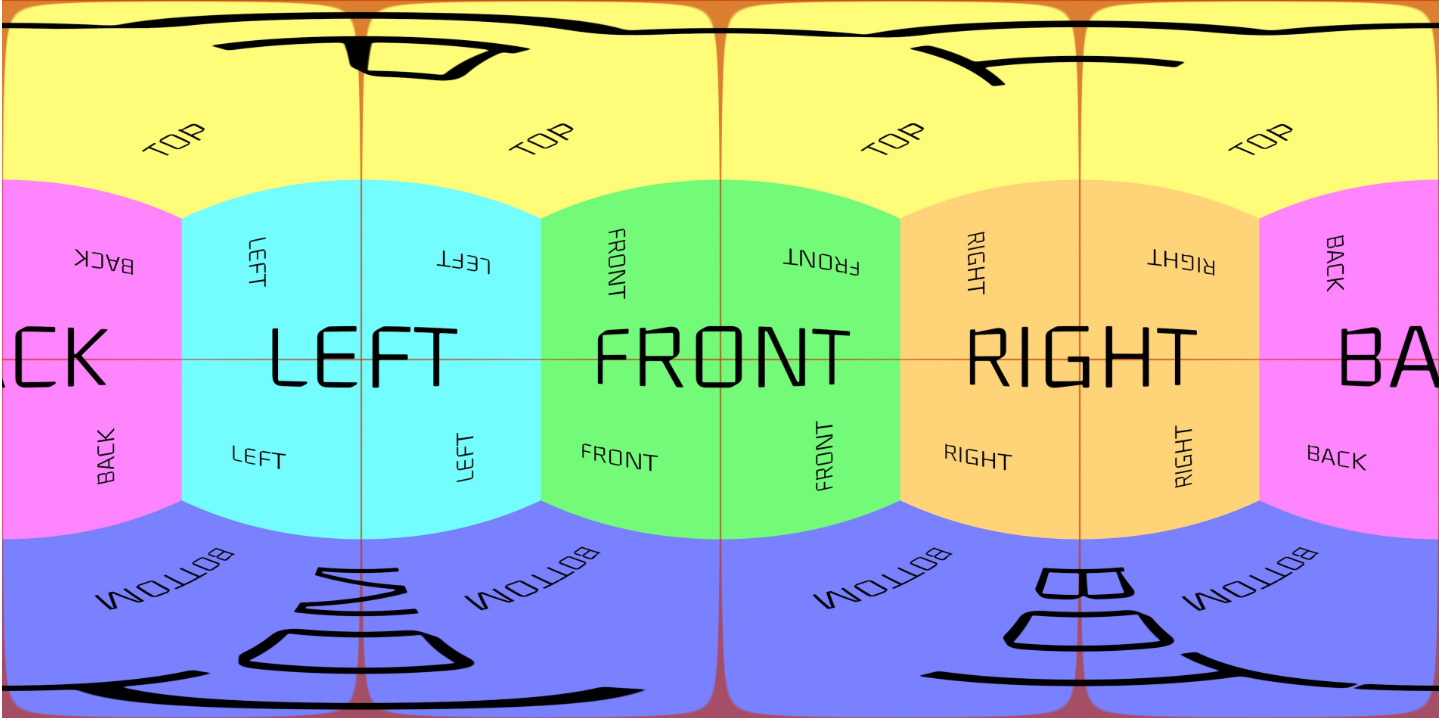
\includegraphics[width=0.8\textwidth]{img/fig_equirectangular.png}
            \caption{等距柱状投影原理示意图：球面经纬度展开为平面坐标}
            \label{fig:equirectangular}
        \end{figure}

        结合图 \ref{fig:equirectangular}，我深入理解了球体纹理映射的数学本质：即将球面上任意一点的方向向量 $(x, y, z)$ 转换为球坐标系下的经纬度 $(\phi, \theta)$，进而线性映射到平面纹理的 $(u, v)$ 坐标系中。
        
        \item \textbf{工程实践}：掌握原理后，我利用 AI 绘图工具（如 Nanobanana）生成了严谨符合 $2:1$ 比例规范的公园全景图。
        
        \begin{figure}[H]
            \centering
            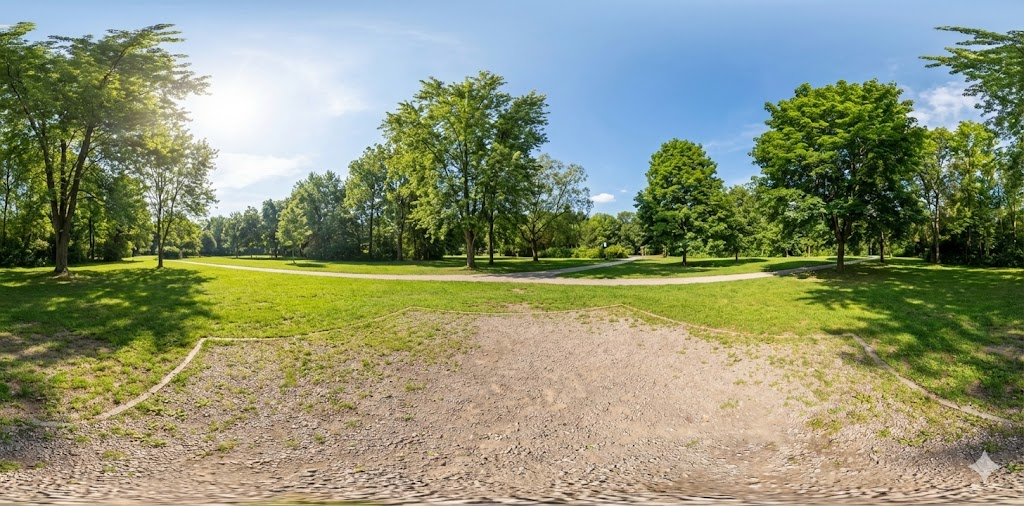
\includegraphics[width=0.8\textwidth]{img/park_scene.jpg}
            \caption{生成的符合等距柱状投影规范的公园全景图}
            \label{fig:park_scene}
        \end{figure}

        \item \textbf{结果}：最终在 Fragment Shader 中，利用 GLSL 的反三角函数（\texttt{atan} 和 \texttt{asin}）实现了精确的纹理采样算法。配合坐标轴的矫正，完美实现了肉眼 3D 的环境包裹效果，消除了接缝与拉伸。
    \end{itemize}

    \item \textbf{文档撰写中的理论可视化挑战}
    \begin{itemize}
        \item \textbf{遭遇问题}：在负责撰写实验报告的“理论基础”章节时，我发现仅靠枯燥的文字难以清晰阐述复杂的图形学算法，特别是 Phong 光照模型中高光的计算原理以及 MVP 变换管线的几何意义。
        
        \item \textbf{理论研究与素材搜集}：为了准确表达，我深入复习了 OpenGL 的坐标变换机制，并整理了相关可视化素材。
        
        \begin{figure}[H]
            \centering
            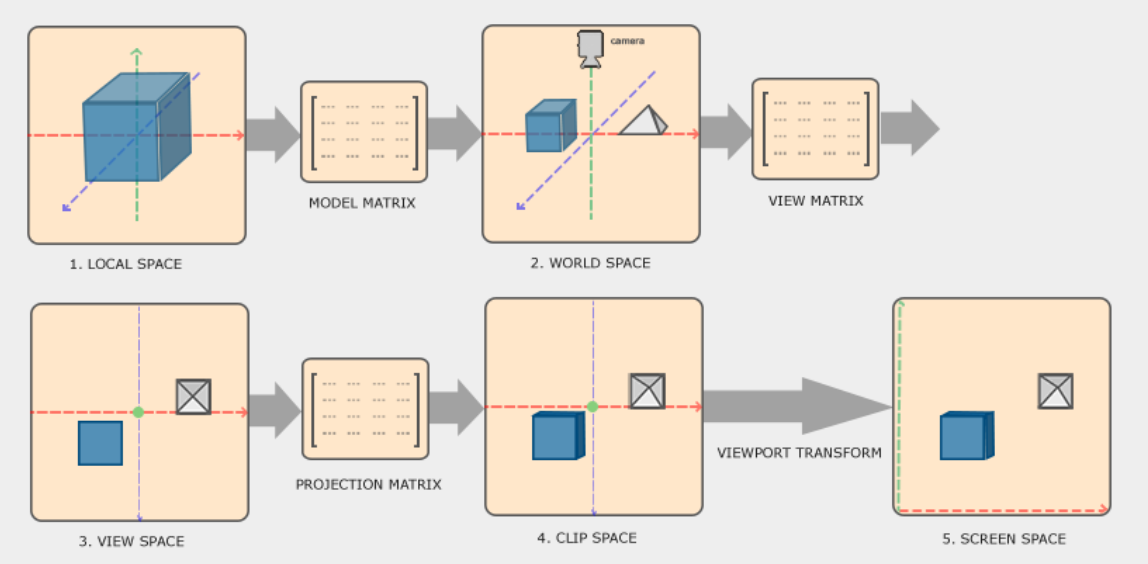
\includegraphics[width=0.9\textwidth]{img/fig_pipeline.png}
            \caption{OpenGL 坐标变换管线：从局部空间到屏幕空间的流转}
            \label{fig:pipeline}
        \end{figure}

        \item \textbf{分析}：通过图 \ref{fig:pipeline}，我理清了顶点从局部空间（Local Space）经由模型、观察、投影矩阵变换到裁剪空间，最后通过透视除法（Perspective Division）到达标准化设备坐标（NDC）的完整链条。这一分析过程确保了报告理论描述的严谨性。
        
        \item \textbf{光照模型深化}：在解释 Phong 模型中的镜面反射（Specular）分量时，为了推导反射向量 $R$ 的计算公式，我引入了向量几何示意图。
        
        \begin{figure}[H]
            \centering
            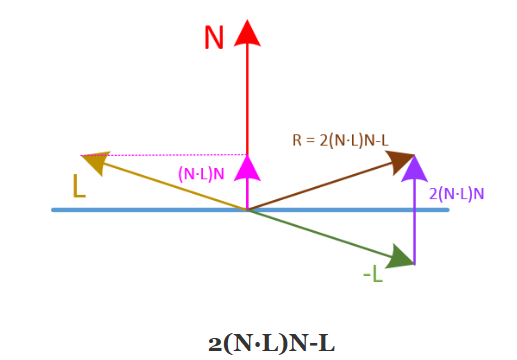
\includegraphics[width=0.5\textwidth]{img/fig_reflection.png}
            \caption{镜面反射向量推导示意图}
            \label{fig:reflection}
        \end{figure}

        \item \textbf{结果}：结合图 \ref{fig:reflection}，我在文档中清晰地推导出了 $R = I - 2(N \cdot I)N$（或 $R = 2(N \cdot L)N - L$，取决于入射向量方向定义）的公式。这不仅解释了 Shader 代码中 \texttt{reflect} 函数的数学含义，也显著提升了个人报告的学术深度。
    \end{itemize}

    \item \textbf{无限远背景下的移动违和感}
    \begin{itemize}
        \item \textbf{困难}：最初实现了 WASD 自由漫游相机，但由于天空盒被设定为无穷远，当相机平移时背景纹理保持静止，导致近处的棋盘看起来像是在漂移。
        \item \textbf{解决}：果断废弃自由移动功能，重构为基于 1-4 数字键的预设视角切换系统。这种设计不仅消除了视觉误差，还提升了作为棋类游戏的专注度与实用性。
    \end{itemize}
\end{enumerate}

\section{体会与总结}

通过本次计算机图形学大作业的实践，我不仅掌握了 OpenGL 3.3 核心管线的编程技术，更在从“需求分析”到“工程落地”的完整开发周期中获得了宝贵的经验。以下是我在项目过程中的五点主要体会：

\begin{enumerate}
    \item \textbf{从直观想象到数学实现的跨越}：
    项目初期，我对 Skybox 的理解仅停留在“像 CS1.6 那样贴几张图”的直观层面。但在实际开发中，我深刻认识到图形学的本质是数学。通过研究等距柱状投影（Equirectangular Projection）并将 $3D$ 向量转换为 $(u,v)$ 坐标的过程，我切身体会到了三角函数与线性代数在构建虚拟世界中的核心作用。

    \item \textbf{“以图搜图”的研究型学习方法}：
    在解决技术难题时，单纯的代码调试往往效率低下。本次实验中，我尝试了“问题驱动”的学习路径——例如在遇到天空盒畸变时，通过查找 UV 展开图（Fig. \ref{fig:equirectangular}）来指导 AI 生成正确的纹理资源。这种结合理论图解与 AI 工具（如 Nanobanana）的复合工作流，极大地提升了我的开发效率。

    \item \textbf{虚实结合的团队协作艺术}：
    天空盒虽然提供了无限远的背景，但若缺乏近景承接，物体会有“悬浮感”。在项目中，我负责背景的无限远渲染，而队友吴深荣负责近处物理地板的建模与阴影接收。我们在“虚（天空）”与“实（地面）”的交界处进行了多次调试，最终实现了光影的自然过渡。这让我理解了在大型图形项目中，模块间的视觉一致性比单一模块的实现更为重要。

    \item \textbf{文档撰写是对知识的二次重构}：
    作为文档负责人，在绘制架构图（Fig. \ref{fig:architecture}）和梳理渲染管线（Fig. \ref{fig:pipeline}）的过程中，我被迫跳出具体的代码细节，从全局视角审视整个系统。这种将离散的代码逻辑抽象为系统理论的过程，不仅加深了我对 MVP 变换和光照模型的理解，也锻炼了我将工程实现转化为学术语言的表达能力。
\end{enumerate}
\end{document}
